%1. I erased lines related to mass, but I left all others assuming they were implemented in the code.
%2. It is possible that there are wrong explanations, so please correct them before actually merging.
%3. I tried to use the same font and format as other manual tex file. Please to feel free to alter/edit fonts, format and the text.
%4. I added a few examples including figures, but please feel free to remove them as you prefer. 
%5. In particular, when I compile with the figures, it does not compile by complaining plot files are not found. It compiles without \begin{figure}[h].....\end{figure}.
%6. Also, if the example with the figures are to be included in the manual, depending on the configuration of the figures, {left} {right} \textit{bottom} panels should be altered accordingly. 
%7. I also provide the parameter table in a separate tex file (particle_parameters.txt). One needs to fill in the default value for each variable. And I have not tried to compile with that file, so it may cause some errors when you compile with it. 




\section{Tracer particles}

Tracer particles are to track the Lagrangian evolution of a model fluid using discrete particles. In hydrodynamical simulations based on an Eulerian grid (including CASTRO), thermodynamic variables at a given time are derived by solving the equations of motion of a fluid between cells. Therefore, in this scheme, the physical quantities that we can access to are not discretized quantities at any given position, but rather average values over each cell. However, employing discrete particles, passively advected with the fluid flow, allows us to obtain local instantaneous thermodynamic variables, such as the temperature and the density, at well-defined positions, independent of the spatial resolution, i.e., the spatial cell size. This means that we can follow the evolution of the fluid at any given position and time. 

\noindent CASTRO provides a tracer particle scheme with useful options in which, for example, the number and the initial positions of particles are flexibly determined according to the purpose of a given model. 


\section{Initializing the Particles}

One must include the tracer particles in the {\tt GNUmakefile} by setting

\vspace{0.1in}
\noindent{\tt USE\_PARTICLES = TRUE}.
\vspace{0.1in}

\noindent And the particles can be initialized via

\vspace{0.1in}
\noindent {\tt {\bf castro.do\_tracer\_particles }}     = 1
\vspace{0.1in}

\noindent in the {\tt {\bf inputs}} file.

\vspace{0.1in}
\noindent There are two ways to determine the initial positions of particles on a domain. You can either place the particles manually (Section \ref{particle:manualplacement}) by providing an input file or randomly (Section \ref{particle:randomplacement}) by setting some relavant variables.

\subsection{manually-assigned initial positions}
	\label{particle:manualplacement}
If one wants to investigate the evolution of fluid motions starting from specific positions (or a certain range of area or volume), one can manually specify the positions of particles by providing an input file containing the total number and the initial positions of the particles.  
The input file should be in the same directory where your {\tt inputs} file is located. The name of the input file is  determined via :

\vspace{0.1in}
\noindent {\tt {\bf particles.particle\_init\_file =}}{\em particle\_file}
\vspace{0.1in}

\noindent Here {\em particle\_file} is the user-specified name of the file. The first line in this file is
assumed to contain the number of particles.  Each line after that contains the positions in a coordinate system adopted for your model. For 3-D cartesian coordinates, \\

$x ~y ~z$ \\

For example, an input file for a model fluid with 6 particles in 2-D Cartesian coordinates may look like,\\

\begin{lstlisting}
6
3.28125e+08 9.9198e+08 
5.46875e+08 9.9198e+08 
7.65625e+08 9.9198e+08 
9.84375e+08 9.9198e+08 
1.20312e+09 9.9198e+08 
1.42188e+09 9.9198e+08 
\end{lstlisting}

According to this input file, the 6 particles will be positioned at the same height (same $y$ coordinate in the second column), equally spaced in $x$ direction (the first column except for the particle number on the first line) from $3.28\times10^{8} {\rm ~cm}$ to $1.42\times 10^{9} {\rm ~cm}$.
	
\subsection{randomly-assigned initial positions}
\label{particle:randomplacement}
Alternatively, the positions of particles can be randomly chosen. This may be used to characterize the global movement of a fluid. Even in this way of placing particles, however, the trajectory of each particle can be traced using the index individually assigned to each particle, which can be found in the output file (see Section \ref{particles:output_file}).

To enable this option, set \\

\noindent {\tt {\bf castro.castro.particle\_init\_type = Random}}. \\

\noindent The number of particles are determined by setting: \\

\noindent {\tt {\bf castro.particle\_initrandom\_count = }} particle \# (e.g., 10000).


\section{Particle movement}
%I did not remove this part just in case this is implemented in the code. But if not, please remove it.
\noindent There are currently two different ways in which particles can be moved, random motion and motion by self-gravity.

\noindent To enable the random motion, set \\

\noindent {\tt {\bf castro.particle\_move\_type = Random.}} \\

\noindent This updates the particle positions at the end of each coarse time step using a 
random number between 0 and 1 multiplied by $0.25 \Delta x$ where $\Delta x$ refers to the cell size .


\vspace{0.1in}
\noindent On the other hand, by setting \\

\noindent {\tt {\bf  castro.particle\_move\_type = Gravitational}} \\

the motion of particles are governed by their self-gravity.




\section{Output file}
\label{particles:output_file}
\noindent The output files are stored in a directory whose name is determined by a variable \\
\noindent {\tt particles.timestamp\_dir}. For example, if the variable is set as follows,

\vspace{0.1in}
{\tt  {\bf particles.timestamp\_dir=}} {\em particle\_dir},
\vspace{0.1in}

\noindent A directory {\em particle\_dir} is automatically made with the directories for the main CASTRO output file ({\tt plt****}) once a simulation starts and the particle output files are stored inside that directory.

\vspace{0.05in}
\noindent The name of the output file consists of {\tt Timestamp\_} along with a number at the end. The number increases (typically from 00) as more processors are involved in following the trajectories of particles. In parallel computing, a computational domain is divided according to the number of processors requested. Then each processor only follows the particles on the domain assigned to that processor and records their positions and velocities at any given time in a different output file. Since it is possible for particles to move from one domain to another during the evolution, its history can be stored in different files. More output files (with larger numbers at the end of the file name) can be produced as more processors track the particles. Each particle is characterized by combining the integers in the first two columns in the outpux file, corresponding to a particle index assigned from each processor and the processor number. One way to identify the particles is consider the sum of the two integers as a global index for each particle. 

\vspace{0.05in}
\noindent By default, the output file constains the positions and velocities of all particles at a given time, meaning [$3+ 2\times$dimensionality] columns. For example, for particles in a 3-D domain, the columns in the output file are, 

\vspace{0.1in}
${\rm index1}~~{\rm index2}~~x~~ y~~ z~~ t~~ v_{\rm x} ~~v_{\rm y}~~ v_{\rm z}~~ [\rho ~~ T]$
\vspace{0.1in}

\noindent The first two integers, as mentioned above, correspond to the particle index and the processor number. By setting the following,

\vspace{0.1in}
\noindent {\tt {\bf particles.timestamp\_temperature }}= 1,\\
\noindent {\tt  {\bf  particles.timestamp\_density}}     = 1,
\vspace{0.1in}

\noindent one can also add the last two columns with the local temperature and local density at the particle positions, i.e. $[\rho ~~ T]$. For example, let's consider 10 particles on a domain.  If 4 out 10 particles are initially on a processor and the rest are on another processor, this means two processors are tracking the particles and two output files are produced. In the output file written by the processor with 4 particles, one can find that four lines are stored at the same time and each line corresponds to each particle info. while in the other output file for the other 6 particles, 6 lines are stored at the same time. 



\vspace{0.05in}

\noindent If {\tt {\bf particles.write\_in\_plotfile=1}}, the particle data are stored in a binary file along with the main CASTRO output plotfile in directories {\tt plt*****/Tracer/}. 
\vspace{0.05in}


\noindent The output profile can be post-processed by users. We shows plots below made from the output file as an example.

\begin{figure}[h]
	\centering
	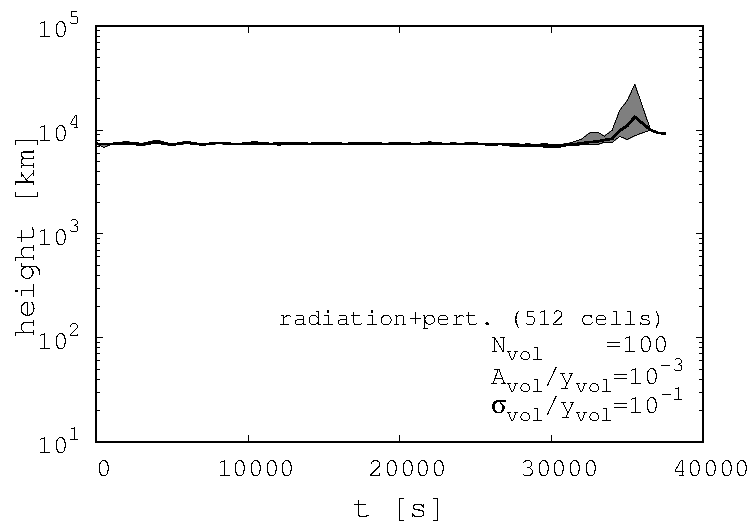
\includegraphics[width=2.1in]{tracerparticleaverage}
	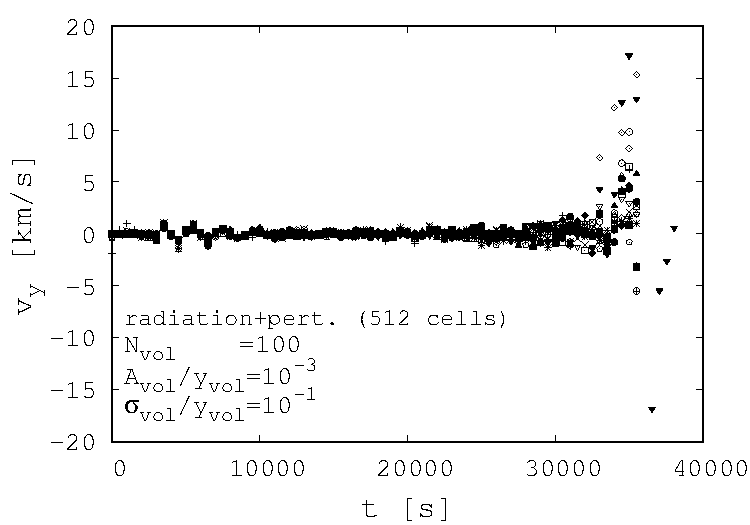
\includegraphics[width=2.1in]{tracerparticleeachvy}
	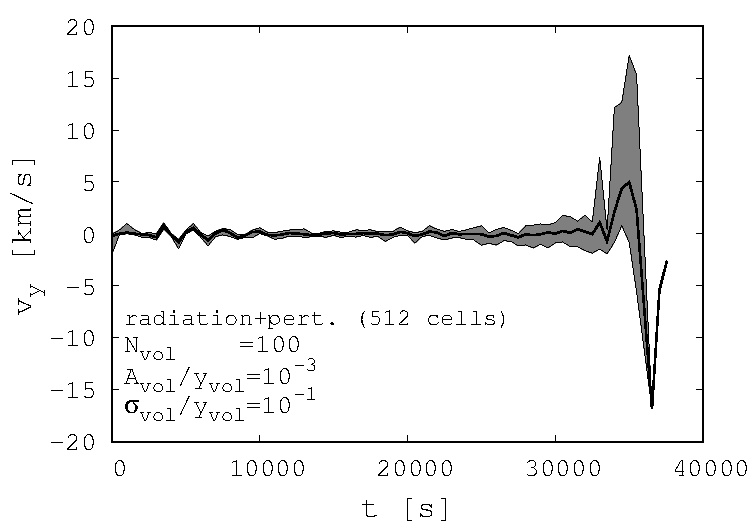
\includegraphics[width=2.1in]{tracerparticlevyaverage}
	\caption{These plots show an example of how the output data can be post-processed and visualized for particles advected with a fluid motion in a model planetary atmosphere. The initial position of the data are given via an input file (Section \ref{particle:manualplacement}) 
		\textit{Left} panel : the time evolution of the heights of particles. The solid line represents the average height and the shaded regions indicate the maximum and minimum values of the height for all particles at a given time. \textit{Right} panel : the velocities in $y$-direction ($v_{\rm y}$) of all particles. Different dot types refer to different particles. \textit{Bottom} panel : same as the \textit{right} panel. However, this shows the average velocity (solid line) and the maximum and minimum velocities at a given time (shaded region). The \textit{left} and \textit{bottom} panels are made after post-processing the data. See perturbation for more detail of the vortex variables ($N_{\rm vol}, A_{\rm vol}$ and $\sigma_{\rm vol}$).}
\end{figure}


\subsection{Run-time Screen Output}

The verbosity written to the screen at run-time is constrolled by setting:

\noindent {\bf particles.v } = 0 or 1 (default: 0)\\


%\end{document}